\documentclass{article}


% if you need to pass options to natbib, use, e.g.:
%     \PassOptionsToPackage{numbers, compress}{natbib}
% before loading neurips_2024


% ready for submission
% \usepackage{neurips_2024}


% to compile a preprint version, e.g., for submission to arXiv, add add the
% [preprint] option:
% \usepackage[nonatbib, preprint]{neurips_2024}


% to compile a camera-ready version, add the [final] option, e.g.:
% \usepackage[nonatbib, final]{neurips_2024}


% to avoid loading the natbib package, add option nonatbib:
\usepackage[nonatbib]{neurips_2024}

\usepackage[utf8]{inputenc} % allow utf-8 input
\usepackage[T1]{fontenc}    % use 8-bit T1 fonts
\usepackage{hyperref}       % hyperlinks
\usepackage{url}            % simple URL typesetting
\usepackage{booktabs}       % professional-quality tables
\usepackage{amsfonts}       % blackboard math symbols
\usepackage{nicefrac}       % compact symbols for 1/2, etc.
\usepackage{microtype}      % microtypography
\usepackage{xcolor}         % colors
\usepackage[numbers]{natbib}
\usepackage[ruled]{algorithm2e}
\usepackage{amsmath}
\usepackage{multicol}
\usepackage{tikz}
\usepackage[dvipsnames]{xcolor}
\usepackage{hhline}
\usepackage{booktabs}
\usepackage{float}
\graphicspath{{../figures/}}
\definecolor{myblue}{RGB}{74, 144, 226}
\definecolor{myred}{RGB}{255, 2, 27}

\title{Rank Reduction Autoencoders - Enhancing interpolation on nonlinear manifolds.}


% The \author macro works with any number of authors. There are two commands
% used to separate the names and addresses of multiple authors: \And and \AND.
%
% Using \And between authors leaves it to LaTeX to determine where to break the
% lines. Using \AND forces a line break at that point. So, if LaTeX puts 3 of 4
% authors names on the first line, and the last on the second line, try using
% \AND instead of \And before the third author name.


\author{%
  Jad Mounayer\\
  ENSAM Institute of Technology\\
  PIMM, SKF Chair\\
  Blvd de l'Hôpital, Paris \\
  \texttt{jad.mounayer@outlook.com}\\
  % examples of more authors
  \And
  Sebastian Rodriguez\\
  ENSAM Institute of Technology\\
  PIMM, RTE Chair\\
  Blvd de l'Hôpital, Paris\\
  \texttt{sebastian.rodriguez\_iturra@ensam.eu}\\
  \AND
  Chady Ghnatios \\
  ENSAM Institute of Technology\\
  PIMM, SKF Chair\\
  Blvd de l'Hôpital, Paris\\
  \texttt{chady.ghnatios@ensam.eu}\\
  \And
  Charbel Farhat \\
  Department of Aeronautics and Astronautics,\\ Stanford University,\\
  Stanford, 94305,\\
  \texttt{cfarhat@stanford.edu}\\
  \And
  Francisco Chinesta \\
  ENSAM Institute of Technology\\
  PIMM, ESI/Keysight Chair\\
  CNRS@CREATE, Singapore\\
  Blvd de l'Hôpital, Paris\\
  \texttt{francisco.chinesta@ensam.eu} \\
}


\begin{document}


\maketitle


\begin{abstract}
    The efficiency of classical Autoencoders (AEs) is limited in many practical situations. When the latent space is reduced through autoencoders, feature extraction becomes possible. However, overfitting is a common issue, leading to 'holes' in AEs' interpolation capabilities. On the other hand, increasing the latent dimension results in a better approximation with fewer non-linearly coupled features (e.g., Koopman theory or kPCA), but it doesn't necessarily lead to dimensionality reduction, which makes feature extraction problematic. As a result, interpolating using Autoencoders gets harder. In this work, we introduce the Rank Reduction Autoencoder (RRAE), an autoencoder with an enlarged latent space, which is constrained to have few dominant singular values (i.e., low-rank). The latent space of RRAEs is large enough to enable accurate predictions while enabling efficient feature extraction. As a result, the proposed autoencoder features a minimal rank linear latent space. To achieve what's proposed, two formulations are presented, a strong and a weak one, that builds a reduced basis that accurately represents the latent space. The first formulation consists of a truncated SVD in the latent space, while the second one adds a penalty term to the loss function. We show the efficiency of our formulations by using both of them for interpolation tasks and comparing the results to state-of-the-art autoencoders.
\end{abstract}

\section{Introduction}\label{sec:intro}
Interpolation of vector functions over a parametric space is an active research topic since accurate interpolation allows the reconstruction of a physical solution in an entire parametric space from a set of pre-computed samples. Multiple techniques have been proposed to perform interpolation, mainly the Proper Orthogonal Decomposition with Interpolation (PODI) \citep{tezzele2019shape, nguyen2022efficient, rama2020towards}, or the sparse-PGD (sPGD) \cite{chinesta2011short, sancarlos2023regularized}. Most of these techniques are based on Model Order Reductions, such as the Proper Orthogonal Decomposition (POD) \cite{rowley2004model, kerschen2005method}, the Proper Generalized Decomposition (PGD) \cite{ladeveze1985famille,rodriguez2019non, chinesta2014pgd}, and the Principal Component Analysis (PCA) \cite{labrin2020principal, gonzalez2018kpca}. These techniques stack the vector functions in what is called the solution matrix, and their efficiency is inversely proportional to the rank of this matrix. If the solution matrix only has a few dominant singular values (i.e., low-rank), the aforementioned techniques can efficiently reduce the problem and interpolate. However, when this assumption does not apply, they fail to define an efficient surrogate for the correct prediction of physical phenomena. A high-rank solution matrix is also problematic for other techniques based on different formulations such as those based on Grassmann manifolds \cite{grasmanian_interp}, the Optimal Transport (OT) \cite{TORREGROSA202212, TORREGROSA202236}, or every low-rank technique (e.g. \cite{srebro2003weighted, liu2012robust, udell2016generalized, davenport2016overview}).

On the other hand, autoencoders with Neural Networks as their encoding and decoding functions are tempting to use for interpolation because of their ability to capture nonlinear behavior. They have been used in different applications such as speech recognition \cite{vachhani2017deep, feng2014speech}, medical applications \cite{deng2019towards}, robotics \cite{park2018multimodal}, and others \cite{bank2023autoencoders}. Yet, the efficiency of Vanilla Autoencoders is limited. On the one hand, Autoencoders with reduced latent spaces (or Diabolo Autoencoders (DAEs)), can easily overfit the data and hence are known for having ``holes'' in their latent spaces. On the other hand, even though enlarged latent spaces lead to better approximations with less non-linear behavior (by the Koopman theory or the kPCA), the representations learned are usually of a large dimension which limits both interpolation and feature extraction. 

% This has led to multiple enhancements such as Variational \cite{doersch2016tutorial}, or Sparse Autoencoders \cite{ng2011sparse} which improved Autoencoders overall but did not definitively solve the interpolation issues.

Neural Networks are increasingly being used for nonlinear reduction techniques \cite{barnett2022neuralnetworkaugmented}. Recently, the Implicit Rank-Minimizing Autoencoder (IRMAE) \cite{jing2020implicit}, and the Low-Rank Autoencoder (LoRAE) \cite{mazumder2023learning} showcased how increasing the latent space dimension while encouraging a low-rank achieves better results, including interpolation. If the latent space has a low rank, the efficiency of all presented interpolation techniques (including basic linear interpolation) in the latent space is enhanced. The resulting Autoencoder would benefit from the large data dimensionality of the latent space to find better approximations while allowing feature extraction because of its low rank. The architecture of IRMAE consists of adding linear layers between the encoder and the latent space, while LoRAE only adds one linear layer as well as its nuclear norm as a penalty for the loss. While both papers show how their resulting latent spaces have a lower rank compared to Vanilla and Variational Autoencoders, their work has some limitations. First, while both architectures can find a low-rank latent space with singular values that are sharply decreasing, they do not force the small singular values to go to zero. Accordingly, the decoder always has some noise from the small singular values, even though ideally, we would like to remove their effect entirely. In addition, the computational time of both architectures highly depends on the latent space dimension $L$. Since a long latent space is crucial for achieving better results, both IRMAEs and LoRAEs can be computationally expensive. Finally, both architectures do not provide explicit control over the rank of the latent space. While they have tuning parameters, we show later in the paper that their proposed parameters can not reach a rank that is as low as we desire.

In this paper, we present Rank Reduction Autoencoders (RRAEs), which have large latent spaces restricted to have a low rank. By enforcing the latent space to accept a linear reduction (hence a lower rank), we show that our model resolves the issues previously mentioned. Our architecture includes two proposed formulations: (i) a strong and (ii) a weak one. Throughout the paper, we show that the strong formulation finds orthogonal basis vectors and forms a reduced POD basis, while the weak formulation is allowed to find non-orthogonal ones. We show that both formulations can interpolate efficiently between high-rank synthetic solutions while achieving a lower rank than the IRMAE and the LoRAE. We also demonstrate how both formulations can overcome other architectures when interpolating over the MNIST dataset, with a significantly lower rank.

The present paper is structured as follows: section \ref{sec:HT} presents the architecture and both proposed formulations. Section \ref{sec:insights} explains the insights behind long latent spaces with a low rank on two synthetic examples. Then, we compare the interpolation capabilities of RRAEs with IRMAEs, and LoRAEs on a variety of problems in section \ref{sec:Nuemrical}. We explain the limitations of the proposed formulations in section \ref{sec:limitations}, before finally summarizing the main original contributions of the present paper in section \ref{sec:conclusions}.

\section{Rank Reduction Autoencoders (RRAEs)}\label{sec:HT}
To define the architecture of RRAEs, we begin by defining autoencoder notations. Let $\{X_i\}_{i\in [1, D]} \in \mathbb{R}^T$ be a set of $D$ series of observations, each having $T$ degrees of freedom. We define our input $X\in \mathbb{R}^{T\times D}$ with $X_i$ as its $i$th column. Let, $Y \in \mathbb{R}^{L\times D}$, with $L$, the chosen dimension\footnote[1]{See Appendix \ref{apdx:train} for details on the choice of $L$.} of the latent space. We also define the encoding map $e: \mathbb{R}^{T\times D} \xrightarrow{} \mathbb{R}^{L\times D}$ and the decoding map $d: \mathbb{R}^{L\times D} \xrightarrow{} \mathbb{R}^{T\times D}$. The Vanilla autoencoder can be written as the following two operations,
\begin{equation}
    Y = e(X), \qquad \tilde{X} = d(Y).
\end{equation}
In practice, we usually enforce that the output of the autoencoder gives us back the original data, hence the loss $\mathcal{L}$ usually reads,
\begin{equation}
    \mathcal{L}(X, \tilde{X}) = \Vert X-\Tilde{X}\Vert_2, \quad \text{where,} \quad \Vert \cdot\Vert_2 \text{ is the $L2$-norm}.
\end{equation}
The idea behind RRAEs is to enforce the latent matrix to have a low rank while finding a reduced basis. In other words, if $Y$ has a rank $r$, let $Y = U\Sigma V$ be the Singular Value Decomposition (SVD) \cite{stewart1993early, nakatsukasa2017accuracy} of $Y$, with $U\in\mathbb{R}^{L\times r}$, $\Sigma \in\mathbb{R}^{r\times r}$, and $V\in\mathbb{R}^{r\times D}$. Let $\{\sigma_i\}_{i \in [1, r]}$ be the sorted diagonal values of $\Sigma$. Thus, by considering the $k$ most significant modes (choice of $k$ detailed in Appendix \ref{apdx:train}), it results,
\begin{equation}\label{eqn:trunc}
    Y = \sum_{i=1}^r\sigma_iU_iV_i^T \qquad\Rightarrow\qquad Y\approx \sum_{i=1}^k\sigma_iU_iV_i^T, \qquad k\ll r,
\end{equation}
where $U_i$ is the $i$th column of $U$ and $V_i^T$ is the $i$th row of $V$. In other words, we can write $Y_d$, the $d$th column of $Y$ as,
\begin{equation}\label{eqn:alphas}
    Y_d \approx \sum_{i=1}^k\left(\sigma_iU_iV_i^T\right)_d = \sum_{i=1}^k\sigma_iU_iV_{i,d} = \sum_{i=1}^k\alpha_{i,d}U_i, \qquad\quad \forall d \in [1, D],
\end{equation}
with $V_{i,d}$ being entry $d$ of vector $V_i^T$.

Accordingly, for $k$ modes, each column of $Y$ is defined by $k$ coefficients and $k$ vectors. Further, vectors $U_i$ form a basis for the latent space. We can write \eqref{eqn:alphas} in matrix form as follows,
\begin{equation}\label{eqn:mat_form}
    Y \approx UA, \qquad \text{with: } A_{i,j}=\alpha_{i,j}, \quad U \in \mathbb{R}^{L\times k}. \quad A \in \mathbb{R}^{k\times D},
\end{equation}
Based on \eqref{eqn:alphas}, and \eqref{eqn:mat_form}, we propose two formulations that enforce the low rank of the latent space and find its reduced basis. The architecture is sketched in Figure \ref{fig:mdoel_arch}.
\tikzset{every picture/.style={line width=0.75pt}} %set default line width to 0.75pt 


\begin{figure}



    \tikzset{every picture/.style={line width=0.75pt}} %set default line width to 0.75pt        

    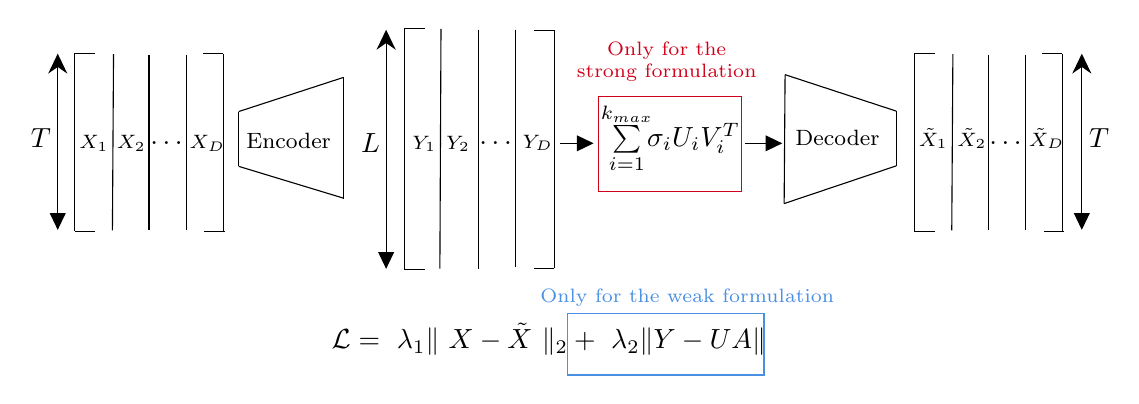
\begin{tikzpicture}[x=0.75pt,y=0.75pt,yscale=-1,xscale=1, scale=0.9]
        %uncomment if require: \path (0,329); %set diagram left start at 0, and has height of 329

        %Straight Lines [id:da21499615368111846] 
        \draw    (37,108.56) -- (37,203.67) ;
        %Straight Lines [id:da16326946357296768] 
        \draw    (37,108.56) -- (47.89,108.56) ;
        %Straight Lines [id:da16265931324232152] 
        \draw    (37,203.67) -- (47.89,203.67) ;
        %Straight Lines [id:da5083389594267504] 
        \draw    (116.56,204.33) -- (116.56,108.67) ;
        %Straight Lines [id:da3615318503641125] 
        \draw    (117.22,203.7) -- (106.33,203.7) ;
        %Straight Lines [id:da9354769223516279] 
        \draw    (116.22,108.6) -- (105.33,108.6) ;
        %Straight Lines [id:da9284204806788381] 
        \draw    (57.67,108.87) -- (57.07,203.27) ;
        %Straight Lines [id:da9687380676381745] 
        \draw    (76.67,109.25) -- (76.67,203.25) ;
        %Straight Lines [id:da30039595434321] 
        \draw    (96.67,109.25) -- (96.67,203.25) ;
        %Straight Lines [id:da782396384119824] 
        \draw    (124.67,139.67) -- (180.67,121.42) ;
        %Straight Lines [id:da9238744798761502] 
        \draw    (124.67,169) -- (180.67,186) ;
        %Straight Lines [id:da44599235940336523] 
        \draw    (180.67,121.42) -- (180.67,186.33) ;
        %Straight Lines [id:da6964885949042201] 
        \draw    (213.3,95.06) -- (213.3,224.17) ;
        %Straight Lines [id:da06959562543054565] 
        \draw    (213.3,95.06) -- (224.19,95.06) ;
        %Straight Lines [id:da030633764479459424] 
        \draw    (213.3,224.17) -- (224.19,224.17) ;
        %Straight Lines [id:da3263511981591738] 
        \draw    (293.52,223.5) -- (293.52,96.17) ;
        %Straight Lines [id:da40502884422960217] 
        \draw    (293.52,223.5) -- (282.63,223.5) ;
        %Straight Lines [id:da8961788198500589] 
        \draw    (293.52,96.3) -- (282.63,96.3) ;
        %Straight Lines [id:da9774520960600939] 
        \draw    (232.97,95.37) -- (232.37,223.77) ;
        %Straight Lines [id:da5075505519042733] 
        \draw    (252.97,95.75) -- (252.97,223.75) ;
        %Straight Lines [id:da21045855349115494] 
        \draw    (272.97,95.75) -- (272.97,222.75) ;
        %Straight Lines [id:da754710144489299] 
        \draw    (124.67,139.67) -- (124.67,169) ;
        %Straight Lines [id:da7099185888654047] 
        \draw    (417.17,119.92) -- (476.67,139.42) ;
        %Straight Lines [id:da66143724081499] 
        \draw    (476.67,168.75) -- (416.67,188.92) ;
        %Straight Lines [id:da31064466545771574] 
        \draw    (417.17,119.92) -- (416.67,188.92) ;
        %Straight Lines [id:da5393972903258972] 
        \draw    (476.67,139.42) -- (476.67,168.75) ;
        %Straight Lines [id:da022156106633165695] 
        \draw    (296.67,156.67) -- (311.67,156.67) ;
        \draw [shift={(314.67,156.67)}, rotate = 180] [fill={rgb, 255:red, 0; green, 0; blue, 0 }  ][line width=0.08]  [draw opacity=0] (8.93,-4.29) -- (0,0) -- (8.93,4.29) -- cycle    ;
        %Straight Lines [id:da38115442380124565] 
        \draw    (395.67,156.67) -- (410.67,156.67) ;
        \draw [shift={(415.67,156.67)}, rotate = 180] [fill={rgb, 255:red, 0; green, 0; blue, 0 }  ][line width=0.08]  [draw opacity=0] (8.93,-4.29) -- (0,0) -- (8.93,4.29) -- cycle    ;
        %Shape: Rectangle [id:dp7709069667907207] 
        \draw  [color={rgb, 255:red, 208; green, 2; blue, 27 }  ,draw opacity=1 ] (317.4,131.47) -- (393.67,131.47) -- (393.67,182.67) -- (317.4,182.67) -- cycle ;
        %Shape: Rectangle [id:dp24666081940562967] 
        \draw  [color={rgb, 255:red, 74; green, 144; blue, 226 }  ,draw opacity=1 ] (300.6,248) -- (405.89,248) -- (405.89,280.67) -- (300.6,280.67) -- cycle ;
        %Straight Lines [id:da9073615867889311] 
        \draw    (27.8,111.67) -- (27.8,200) ;
        \draw [shift={(27.8,203)}, rotate = 270] [fill={rgb, 255:red, 0; green, 0; blue, 0 }  ][line width=0.08]  [draw opacity=0] (8.93,-4.29) -- (0,0) -- (8.93,4.29) -- cycle    ;
        \draw [shift={(27.8,108.67)}, rotate = 90] [fill={rgb, 255:red, 0; green, 0; blue, 0 }  ][line width=0.08]  [draw opacity=0] (10.72,-5.15) -- (0,0) -- (10.72,5.15) -- (7.12,0) -- cycle    ;
        %Straight Lines [id:da1988310735559562] 
        \draw    (203.6,98.87) -- (203.6,220.87) ;
        \draw [shift={(203.6,223.87)}, rotate = 270] [fill={rgb, 255:red, 0; green, 0; blue, 0 }  ][line width=0.08]  [draw opacity=0] (8.93,-4.29) -- (0,0) -- (8.93,4.29) -- cycle    ;
        \draw [shift={(203.6,95.87)}, rotate = 90] [fill={rgb, 255:red, 0; green, 0; blue, 0 }  ][line width=0.08]  [draw opacity=0] (10.72,-5.15) -- (0,0) -- (10.72,5.15) -- (7.12,0) -- cycle    ;
        %Straight Lines [id:da7075949415859115] 
        \draw    (486.33,108.56) -- (486.33,203.67) ;
        %Straight Lines [id:da776447423867771] 
        \draw    (486.33,108.56) -- (497.22,108.56) ;
        %Straight Lines [id:da40114415684531135] 
        \draw    (486.33,203.67) -- (497.22,203.67) ;
        %Straight Lines [id:da24114735322590564] 
        \draw    (565.89,204.33) -- (565.89,108.67) ;
        %Straight Lines [id:da8606039915940866] 
        \draw    (566.56,203.7) -- (555.67,203.7) ;
        %Straight Lines [id:da6175875067439736] 
        \draw    (565.56,108.6) -- (554.67,108.6) ;
        %Straight Lines [id:da9114789567469446] 
        \draw    (507,108.87) -- (506.4,203.27) ;
        %Straight Lines [id:da9606142652454763] 
        \draw    (526,109.25) -- (526,203.25) ;
        %Straight Lines [id:da3463806230867499] 
        \draw    (546,109.25) -- (546,203.25) ;
        %Straight Lines [id:da3635085614733373] 
        \draw    (576.02,111.67) -- (576.02,200) ;
        \draw [shift={(576.02,203)}, rotate = 270] [fill={rgb, 255:red, 0; green, 0; blue, 0 }  ][line width=0.08]  [draw opacity=0] (8.93,-4.29) -- (0,0) -- (8.93,4.29) -- cycle    ;
        \draw [shift={(576.02,108.67)}, rotate = 90] [fill={rgb, 255:red, 0; green, 0; blue, 0 }  ][line width=0.08]  [draw opacity=0] (10.72,-5.15) -- (0,0) -- (10.72,5.15) -- (7.12,0) -- cycle    ;

        % Text Node
        \draw (38,151.2) node [anchor=north west][inner sep=0.75pt]  [font=\scriptsize]  {$X_{1}$};
        % Text Node
        \draw (58,151.2) node [anchor=north west][inner sep=0.75pt]  [font=\scriptsize]  {$X_{2}$};
        % Text Node
        \draw (97,151.2) node [anchor=north west][inner sep=0.75pt]  [font=\scriptsize]  {$X_{D}$};
        % Text Node
        \draw (127.33,149.67) node [anchor=north west][inner sep=0.75pt]  [font=\footnotesize] [align=left] {Encoder};
        % Text Node
        \draw (216.3,151.23) node [anchor=north west][inner sep=0.75pt]  [font=\scriptsize]  {$Y_{1}$};
        % Text Node
        \draw (234.3,151.23) node [anchor=north west][inner sep=0.75pt]  [font=\scriptsize]  {$Y_{2}$};
        % Text Node
        \draw (275.3,150.73) node [anchor=north west][inner sep=0.75pt]  [font=\scriptsize]  {$Y_{D}$};
        % Text Node
        \draw (421.33,148.17) node [anchor=north west][inner sep=0.75pt]  [font=\footnotesize] [align=left] {Decoder};
        % Text Node
        \draw (301,101.2) node [anchor=north west][inner sep=0.75pt]  [font=\scriptsize,color={rgb, 255:red, 208; green, 2; blue, 27 }  ,opacity=1 ] [align=left] {\begin{minipage}[lt]{69.37pt}\setlength\topsep{0pt}
                \begin{center}
                    Only for the \\strong formulation
                \end{center}

            \end{minipage}};
        % Text Node
        \draw (284.8,233.2) node [anchor=north west][inner sep=0.75pt]  [font=\scriptsize,color={rgb, 255:red, 74; green, 144; blue, 226 }  ,opacity=1 ] [align=left] {Only for the weak formulation};
        % Text Node
        \draw (12,147.6) node [anchor=north west][inner sep=0.75pt]    {$T$};
        % Text Node
        \draw (188.8,149.8) node [anchor=north west][inner sep=0.75pt]    {$L$};
        % Text Node
        \draw (317.2,134) node [anchor=north west][inner sep=0.75pt]    {$\sum \limits_{i=1}^{k_{max}} \hspace{-0.13cm}\sigma _{i} U_{i} V_{i}^{T}$};
        % Text Node
        \draw (173.07,251.73) node [anchor=north west][inner sep=0.75pt]    {$\mathcal{L} =\ \lambda _{1} \| \ X-\tilde{X} \ \Vert _{2} +\ \lambda _{2} \| Y-UA\Vert $};
        % Text Node
        \draw (76,154.07) node [anchor=north west][inner sep=0.75pt]    {$\dotsc $};
        % Text Node
        \draw (252.13,154.07) node [anchor=north west][inner sep=0.75pt]    {$\dotsc $};
        % Text Node
        \draw (487.33,147.2) node [anchor=north west][inner sep=0.75pt]  [font=\scriptsize]  {$\tilde{X}_{1}$};
        % Text Node
        \draw (525.13,154.07) node [anchor=north west][inner sep=0.75pt]    {$\dotsc $};
        % Text Node
        \draw (508,147.2) node [anchor=north west][inner sep=0.75pt]  [font=\scriptsize]  {$\tilde{X}_{2}$};
        % Text Node
        \draw (546.33,147.2) node [anchor=north west][inner sep=0.75pt]  [font=\scriptsize]  {$\tilde{X}_{D}$};
        % Text Node
        \draw (578.56,147.6) node [anchor=north west][inner sep=0.75pt]    {$T$};


    \end{tikzpicture}

    \caption{Schematic showing the autoencoder in use as well as both methodologies. There are two terms in the loss function for the \textcolor{myblue}{Weak formulation}. On the other hand, there's an additional step before the decoder for the \textcolor{myred}{Strong formulation}.}
    \label{fig:mdoel_arch}
\end{figure}

\begin{enumerate}
    \item \underline{The Weak formulation:} After choosing the maximum allowed number of modes $k_{max}$, we generate two trainable matrices $A \in \mathbb{R}^{k_{max}\times D}$, and $U \in \mathbb{R}^{L\times k_{max}}$. Afterward, we add a term to the loss as seen in blue in Figure \ref{fig:mdoel_arch}. By doing so, minimizing the loss means that the latent space would have at most a rank of $k_{max}$. After convergence, the columns of our trainable matrix $U$ form the reduced basis of the latent space. Additionally, the coefficients found in matrix $A$ describe how to reconstruct each column $Y_d$ as a linear combination of the basis vectors. We will refer to this method as the Weak formulation since throughout training, the Network minimizes a sum of both terms and not each term individually. Accordingly, predictions $\tilde{X}$ could be less accurate, and  we might end up with more modes than the specified value of $k_{max}$.

          \underline{Remark:} The two trainable matrices can be computed from a one-rank greedy procedure, as PGD performs.
    \item \underline{The Strong formulation:} Unlike the weak formulation, this architecture enforces, in a strong manner, the maximum dimension of the reduced basis of the latent space. Similarly to the weak formulation, we begin by choosing the maximum rank $k_{max}$ of the latent space. Then, as seen in red in Figure \ref{fig:mdoel_arch}, a truncated SVD (of order $k_{max}$) of the latent space is given to the decoder, instead of the latent space itself. Accordingly, the input of the decoder will have at most $k_{max}$ dominant singular values. We refer to this method as the Strong formulation since we strictly enforce the latent space to have a rank that's lower or equal to $k_{max}$. In this case, the basis vectors and coefficients are simply the ones found by the truncated SVD.
\end{enumerate}

In both formulations, $k_{max}$ is a hyperparameter to be chosen. We propose a strategy to choose this hyperparameter and discuss its effect in Appendix \ref{apdx:train}.

When using the strong formulation, we compute a POD basis since the vectors are by construction orthogonal. The orthogonality of the basis vectors, as well as refraining from adding terms in the loss, can make both the training and interpolation better. On the other hand, backpropagation through the singular value decomposition is not common in practice. All the work presented in this paper was performed using \texttt{equinox} in \texttt{JAX}, where gradients of the singular value decomposition are implemented and accessible.

Both formulations reduce the limitations of IRMAE and LoRAE. We sum up our contributions as follows:
\begin{enumerate}
    \item RRAEs with a strong formulation lead to low-rank latent spaces that have many singular values exactly equal to zero. In other words, the decoder will get a sum of exactly $k_{max}$ rank-one updates. As will be shown later in the paper, this gives the strong formulation an advantage for training and interpolation.
    \item The computational overhead of RRAEs can be much lower, especially for large latent spaces. For the strong formulation, when batches are used, the SVD is only performed on a matrix of size $L\times bs$, $bs$ being the batch size. Similarly, for the weak formulation, the added computational cost is minimal since the trainable matrices are of shape $L \times k_{max}$ and $k_{max} \times D$ with $k_{max} \ll L$. On the other hand, the IRMAE or the LoRAE either perform a gradient descent or find the nuclear norm of an $L\times L$ matrix. Since a large latent space dimension $L$ usually helps in achieving better results, both IRMAEs and LoRAEs can be computationally challenging. 
    \item Both formulations give us explicit control over the rank of the latent space. As shown next in the paper, we can control the latent space to have a lower rank than IRMAE and LoRAE, which leads to better interpolation and could help for feature extraction in future applications.
\end{enumerate}

% \section{Interpolation in the latent space}\label{sec:interp}
% The fact that motivated us to make this proposal is the limitations of linear interpolation between solutions when the solution matrix is high-rank. Take, for instance, sinusoidal curves shifted by a scalar $p$ (i.e. $\sin(x+p)$). As can be seen in Figure \ref{fig:sin}, interpolating linearly between the curves corresponding to parameters $p_0 = 0$ and $p_1 = \pi$ to find the middle curve at $p^*= \pi/2$ (i.e. simply the sum divided by two) leads to the horizontal line at zero, instead of finding the correct curve shifted towards the middle.


% \begin{figure}[!b]
%     \centering
%     \includegraphics[clip, trim=0.2cm 0.3cm 0cm 1cm, width=0.54\textwidth]{sin.pdf}
%     \caption{Result when interpolating linearly between two shifted sine curves, showing why linear interpolation is not a good choice for problems with multiple dominant singular values.}
%     \label{fig:sin}
% \end{figure}


% By mapping the data into a larger latent space while enforcing a low rank, we can find a space where a linear interpolation would be possible to represent the interpolated curve, before going back to the original space, using the decoder.

% Both proposed formulations allow us to approximate the latent space by \eqref{eqn:alphas}. Now let's suppose that every series of observations $X_d$ is tied to a vector of parameters $\mathbf{p}_d \in \mathbb{R}^P$. Accordingly, and since the basis vectors (i.e. columns of $U$) are the same for any solution, we can interpolate between the coefficients $\alpha_{j,d}$,
% \begin{equation}
%     Y_d=\sum_{j=1}^{k_{max}}\alpha_{j,d}U_j \qquad \Longrightarrow \qquad Y_d(\textbf{p}_d) = \sum_{j=1}^{k_{max}}\gamma_j(\textbf{p}_d)U_j,
% \end{equation}
% where each $\gamma_j: \mathbb{R}^P \xrightarrow{} \mathbb{R}$, could be any mapping, that maps all the training parameters to the corresponding $\alpha_{j,d}$, and allows us to interpolate when used on new values of $\mathbf{p}$. Since we interpolate between coefficients, the computational cost of RRAEs for interpolation is the same as the cost of using a Vanilla Autoencoder with a latent space of dimension $k_{max}$.

% For instance, for a parameter space of dimension one and sorted coefficients, we can interpolate linearly by writing,
% \begin{equation}
%     \gamma_j(p) = \alpha_{j,m} + \frac{\alpha_{j, m+1}-\alpha_{j,m}}{p_{m+1}-p_{m}}(p-p_{m}), \qquad \forall p \in [p_m, p_{m+1}].
% \end{equation}
% In this paper, we show that interpolating linearly for parametric spaces of dimension one, and bilinearly for those of dimension two is enough. In general, each $\gamma_j$ can be approximated by any regression, including a Neural Network, or the sPGD.
\section{Insights behind Long latent spaces with low rank}\label{sec:insights}
An enlarged latent space can exhibit a linear behavior (as employed for instance in the Koopman theory, or the kPCA). Furthermore, a latent space with a reduced basis allows us to interpolate better, as well as extract features. The Diabolo Autoencoder on the other hand has ``holes'' in its interpolation \cite{jing2020implicit}, since it does not find a basis, but only a set of coefficients that are helpful for the decoder to retrieve the solution. Since the decoder is highly nonlinear, the coefficients can be anything, which leads to overfitting.

To illustrate the aforementioned arguments, we test DEAs and our Strong formulation on two examples characterized by one parameter. The first curves we propose are shifted sine curves since these have a simple nonlinearity, but they are hard to separate (nonmonotonic and cross each other multiple times). For our second example, we chose curves with stair-like behavior. In that case, we create highly nonlinear curves (different supports, different numbers of jumps of different magnitudes), but we define them to be monotonic and only cross each other occasionally (i.e. easier to separate). The equations used to define the columns of our input matrix $X$ in each case are as follows,
\begin{equation}\nonumber
    \begin{cases}
        X_d(t_v,\, p_d) = f_{shift}(t_v, \, p_d) = \sin(t_v-p_d\pi), \hspace{0.1cm}\qquad\quad & p_d \in [0, 1.7], \\[1.2ex]
        X_d(t_v, \,p_d) = f_{stair}(t_v,\, p_d, \, \text{args}) \qquad\quad                    & p_d \in [1, 5],
    \end{cases}
\end{equation}
where $t_v \in \mathbb{R}^T$ is a vector of time at which observations are done, and $f_{stair}$ takes some arguments ``args'' as detailed in the algorithm in Appendix \ref{apdx:stair}. Training is performed over 17, and 40 equidistant values of $p_d$ for the shifted sine curves and the stair-like curves respectively. We then interpolate in the latent space of the Autoencoders on 80 and 300 random values of $p_d$, respectively, chosen inside the training domain. The large number of tests guarantees that the models are learning the dynamics and not just the training curves and some tests nearby. Since the solution curves depend on one parameter, we use a DAE with a single scalar latent space and an RRAE with a longer latent space of rank one. We then linearly interpolate in the latent space to predict the test set. The training parameters, including the dimension of the latent space, can be found in Appendix \ref{apdx:train}. The relative error over all $p_d$ values for both the train and test sets is summarized in Table \ref{fig:table_shift_sin}. Further, for each example, predictions over some tests are plotted in Figure \ref{fig:sin_shift_test}.



\begin{table}[!h]
    \caption{Relative error (in \%) for all three architectures on both the train and test sets for both the examples of shifted sin curves and stair-like ones.}
    \label{fig:table_shift_sin}
    \centering
    \begin{tabular}{ccccc}
        \toprule
        {}            & \multicolumn{2}{c}{Shifted sine} & \multicolumn{2}{c}{Stair-like}                                \\
        \cmidrule(lr){2-5}                                                                                               \\
        \addlinespace[-0.2cm]
        Model         & Train Error                      & Test error                     & Train Error   & Test error   \\
        \midrule
        DAE    &    2.12                         & 32.42                          & 2.97          & 3.74         \\
        RRAE (strong) & \textbf{1.73}                    & \textbf{1.90}                   & \textbf{1.87} & \textbf{3.2} \\
        \bottomrule
    \end{tabular}
\end{table}


The results show that when curves are hard to separate, RRAEs are better interpolators than DAEs. On the other hand, the effect of longer latent spaces is reduced for simple curves that can be highly nonlinear, but characterized by one parameter, and easily separable.


\begin{figure}[!t]
    \centering
    \includegraphics[clip, scale=0.3, trim=3cm 1cm 0cm 2cm]{sin_shift_plot_test.pdf}
    \caption{Predictions of Vanilla Autoencoders and RRAEs with both formulations over two particular values of $p_d$ for the shifted sine (above) and the stair-like examples (below).}
    \label{fig:sin_shift_test}
\end{figure}


\begin{figure}[!b]
    \centering
    \includegraphics[clip, scale=0.25, trim=-1cm 1cm 0cm 3.2cm]{sin_shift_plot_latent.pdf}
    \caption{Normalized Coefficients to be interpolated (dots) for DAE and RRAE with a strong formulation, and the interpolated values for the test set (crosses) for the shifted sine curves (left) and the stair-like curves (right).}
    \label{fig:sin_shift_latent}
\end{figure}


To further investigate the results, we plot the coefficients to be interpolated in the latent space as a function of the corresponding parameter in Figure \ref{fig:sin_shift_latent}. It is important to note that the coefficients are defined differently between the RRAE and the DAE. For RRAEs, when $k_{max} = 1$,  the coefficients are simply the entries of $A \in \mathbb{R}^D$ in \eqref{eqn:mat_form}. On the other hand, for a Diabolo Autoencoder with a scalar latent space, the values in the latent space themselves are the coefficients.

The main problem with the coefficients found by the DAE for the shifted sine curves (the blue crosses and dots in Figure \ref{fig:sin_shift_latent} (left)) is that the resulting curve from linearly interpolating the coefficients is not an injection, over two significant parts of the domain. Specifically, for any value of $p_d$ in approximately $[0, 0.3]$ and $[1.3, 1.5]$ (the dotted lines), there exists another value with the same coefficient $\alpha$. Accordingly, the decoder will find the same curve for two different parameters, which is wrong since $p_d$ defines a shift. This explains why the DAE can interpolate well in the top left subplot in Figure \ref{fig:sin_shift_test}, but not in the top right one. These results also show what is meant by ``holes'' in the latent space for DAEs.

On the other hand, as proposed earlier, a longer latent space allows us to find better coefficients. This is clearly shown by the coefficients of the strong method in Figure \ref{fig:sin_shift_latent} (left), which have a monotonic behavior.

Finally, the right part of the figure depicts that when the curves are simple to separate and are characterized by only one parameter, both architectures can find monotonic coefficients that fit both the train and test sets. We conclude that even though long latent spaces have many advantages, they are not always necessary, especially when the solution is simple and separable.
\section{Testing on Numerical Data}\label{sec:Nuemrical}
The solutions interpolated in the previous section were only characterized by one parameter. In this section, we test RRAEs and compare them to IRMAEs, and LoRAEs on two examples with a parametric space of dimension two, as well as on the MNIST dataset.
\subsection{Examples with two parameters}\label{sec:numerical_example}
We generated two challenging synthetic tests for interpolation. First, we propose the sum of two sine curves with different frequencies, as well as two Gaussian bumps in two different locations. We show how in such examples both our formulations result in latent spaces with a lower rank and better results than IRMAEs and LoRAEs for the hyperparameters chosen (again, training details can be found in Appendix \ref{apdx:train}). We define the columns of our input matrix $X_d(t_v,\, p_d) = f_{prob}$ for each problem as follows,
\begin{equation}\nonumber
    \begin{cases}
        f_{freqs}(t_v,\, \textbf{p}_d) = \sin(p^1_d\pi t_v)+\sin(p^2_d\pi t_v), \qquad\qquad\quad                       & p^1_d \in [0.3, 0.5], \quad p^2_d \in [0.8, 1], \\[1.5ex]
        f_{gauss}(t_v,\, \textbf{p}_d) =  1.3e^{-\frac{(t_v-p^1_d)^2}{0.08}}+1.3e^{-\frac{(t_v-p^2_d)^2}{0.08}}, \qquad & p^1_d \in [1, 3], \quad p^2_d \in [4, 6],
    \end{cases}
\end{equation}
We distinguish between the \textbf{bold} notation for vectors and non-bold ones for scalars. In both expressions, our parametric space is of dimension $2$ and so $\textbf{p}_d = [p^1_d, \,p^2_d] \in \mathbb{R}^2$. For each example and each architecture, we present some interpolated predictions in Figure \ref{fig:sin_sin_gauss}, and the error over all the training/testing sets in Table \ref{fig:table_sin_sin_gauss} as well as the average training time for 100 batches.


\begin{table}[h]
    \caption{Relative error (in \%) for all architectures on both the train and test with a latent space of dimension 2800 for the two examples presented, as well as the average time (in s) for 100 batches.}
    \label{fig:table_sin_sin_gauss}
    \centering
    \begin{tabular}{cccccc}
        \toprule
        {}            & \multicolumn{2}{c}{Mult. Frequencies} & \multicolumn{2}{c}{Mult. Gausses}                                             \\
        \cmidrule(lr){2-5}                                                      \\
        \addlinespace[-0.2cm]
        Model        & Train Error                       & Test error    & Train Error   & Test error  &  Average time   \\
        \midrule
        RRAE (strong)          & 6.33                      & \textbf{12.83} & \textbf{4.46} & \textbf{8.75} & 1.61\\
        RRAE (weak)         & 10.33                             &     15.09     & 8.50         & 10.69  & \textbf{0.52} \\
        IRMAE (l=2)        & 6.95                             &      17.35    & 4.68         & 13.93 & 3.6\\
        IRMAE (l=4)        &     N/A                         &     N/A     & 8.41         & 14.78 & 7.50\\
        LoRAE        &    \textbf{5.40}                          &    13.83      &          &   & 420.4\\
        \bottomrule
    \end{tabular}
\end{table}

\begin{figure}[!t]
    \centering
    \includegraphics[clip, scale=0.33, trim=1.6cm 1.2cm 0cm 2.4cm]{sin_sin_gauss_plot_test.pdf}
    \caption{Interpolated results of RRAEs with both formulations on both examples presented with bilinear interpolation in the latent space.}
    \label{fig:sin_sin_gauss}
\end{figure}

\begin{figure}[!b]
    \centering
    \includegraphics[clip, scale=0.29, trim=1.6cm 1.3cm 0cm 2.6cm]{sing_vals_gauss.pdf}
    \caption{Normalized singular values of the latent space $Y$ when trained over multiple gausses. The first 40 singular values are shown to the left, while many of the small singular values are shown on a log scale to the right.}
    \label{fig:sin_vals_gauss}
\end{figure}

As can be seen in Table \ref{fig:table_sin_sin_gauss}, both our formulations are outperforming the IRMAE and LoRAE for a fixed choice of hyperparameters. Additionally, we note that increasing the parameter $l$ for the IRMAE leads to divergence of the gradient descent (hence the N/A). Note that we only used the parameters specified in both papers for IRMAE and LoRAE. A fine-tuning of the parameters could lead to better results for these architectures. On the other hand, the table shows how much faster our proposed formulations are. Our formulations are fast since we only add small matrices to the loss in the weak formulation, and we compute an SVD of an $L\times bs$ matrix, $bs$ being the batch size, in the Strong formulation. On the other hand, IRMAEs and LoRAEs find the gradient/the nuclear norm of an $L\times L$ matrix respectively, with $L$ relatively large. 

Additionally, we draw parts of the normalized singular values of the latent space for the multiple gausses problem in figure \ref{fig:sin_vals_gauss}. The figure illustrates that adding the number of linear layers for the IRMAE (i.e. increasing $l$) indeed reduces the rank of the latent space. However, both of our formulations can be asked to find latent spaces with lower ranks. From the log graph to the right, we can understand why the strong formulation achieves the best results. As previously mentioned, the IRMAE, the LoRAE and our weak formulation don't enforce the singular values to fall to zero. So even though many singular values are small, they still have a noise effect over the decoder, which reduces their efficiency in interpolation. On the other hand, the weak formulation does better than both the IRMAE and LoRAE since it enforces a lower rank.

\subsection{Testing on MNIST}\label{sec:extensions}
In this section, we compare our architecture to the IRMAE and the LoRAE on the MNIST dataset. An example of linear interpolation of five steps between numbers $5$ and $0$ can be seen in figure \ref{fig:interp_mnist}. The singular values of the latent space for all formulations can be found in figure \ref{fig:sin_vals_mnist}.

The interpolation in figure \ref{fig:interp_mnist} depicts that the Strong formulation is capable of performing better interpolation. While all techniques face problems with the second subplot from the left, the drawing for the strong formulation is the closest to a $5$, while the drawing for the weak formulation could be confused for a $6$, and the corresponding picture for the IRMAE doesn't look like a number.

On the other hand, the singular values drawn in figure \ref{fig:sin_vals_mnist} show that the weak formulation surprisingly converges to a very low rank. It is important to note that both the strong and the weak formulations were able to interpolate on the MNIST dataset with a rank that's strictly less than 6. This shows the ability of our formulations to perform feature extraction. Again, the noise caused by the nonzero singular values is the main reason behind the enhanced capabilities of the strong method to interpolate between numbers.
\begin{figure}[!b]
    \centering
    \includegraphics[clip, scale=0.6, trim=0 0cm -1cm 1cm]{mnist_interp.pdf}
    \caption{Three-step interpolation between a rotated number $5$ and a number $0$ on MNIST using RRAEs with both formulations, IRMAEs, and LoAREs.}
    \label{fig:interp_mnist}
\end{figure}

\begin{figure}[!t]
    \centering
    \includegraphics[clip, scale=0.29, trim=1.6cm 1.3cm 0cm 2.6cm]{sing_vals_mnist.pdf}
    \caption{Normalized singular values of the latent space $Y$ when trained over MNIST. The first 40 singular values are shown to the left, while many of the small singular values are shown on a log scale to the right.}
    \label{fig:sin_vals_mnist}
\end{figure}

\section{Limitations}\label{sec:limitations}
As has been shown in the paper's results, RRAEs with both formulations can interpolate well while using a latent space with a low rank. However, our proposed model has some limitations:
\begin{enumerate}
    \item Even though both of our formulations allow explicit control over the rank of the latent space, $k_{max}$ is an additional hyperparameter to be tuned. In practice, we found that starting with a small value of $k_{max}$ and increasing it until error convergence is a good strategy. In general, other techniques such as a PCA could be used to approximate the intrinsic dimension of the latent space.
    \item The weak formulation adds regularisation constants to the loss, which can be hard to tune. However, we found that by monitoring the two terms in the loss while training, it is clear in the first few epochs which constant should be increased/decreased. Yet, training should be performed multiple times to tune the weights of each term in the loss.
    \item For high dimensional problems where a very large latent space is needed, the strong formulation can be computationally expensive. Even though the SVD is only performed on a matrix of size $L\times bs$, $bs$ being the batch size and $L$ the length of the latent space, the cost of computing an SVD and backpropagating through it when $L$ is very large can be high.
    \item As shown in Section \ref{sec:insights}, the effect of a long latent space is reduced when the solution is simple and separable. In such cases, an increased dimension of the latent space, hence RRAEs, might not be necessary.
\end{enumerate}

\section{Summary and Conclusions}\label{sec:conclusions}
In this article, we presented Rank Reduction Autoencoders (RRAEs), Autoencoders with latent spaces that accept linear reduction. We proposed two formulations, a weak and a strong one to find the latent space while building its reduced basis. Even though the basis vectors in the strong formulation are orthogonal, and they need not be in the weak formulation, we showed that both formulations can interpolate well between curves. 

Overall, our results show that the Strong formulation has a superior capability of interpolation since it doesn't have any noise from small nonzero singular values in the latent space. We also showed that both the Strong and the Weak formulations can achieve much lower ranks in the latent space and hence can interpolate better than existing methodologies. Finally, both formulations are faster to train, with the weak formulation being the fastest. While the Strong formulation leads to better predictions, the Weak formulation is much simpler to implement since it only adds a penalty term to the loss.
\newpage

\bibliographystyle{plainnat}
\bibliography{sn-bibliography}
\newpage
\appendix
\section{Algorithm for the stair-like function}\label{apdx:stair}
\begin{algorithm}[H]
    \SetKwInput{Input}{Input}
    \SetKwInput{Output}{Output}

    \Input{$p_d\in \mathbb{R}$, $t_v \in \mathbb{R}^T, (\text{Ph}_0, \text{Amp}_0,\kappa, y_0, w) \in \mathbb{R}$}
    ~\\
    $\text{Amp}_{p_d} = p_d$\\[1.6ex]
    $\displaystyle\text{Ph}_{p_d} = \text{Ph}_0+\kappa(\text{Amp}_{p_d}-\text{Amp}_0)$\\[1.6ex]
    $g_{p_d}(t_v) = \text{Amp}_{p_d}\sqrt{t_v}\sin(w(t_v-\text{Ph}_{p_d}))-y_0$\\[1.6ex]
    $\displaystyle h_{p_d}(t) = \left(\frac{\left|g_{p_d}(t)\right|+g_{p_d}(t)}{2}\right)^5$\\[1.6ex]
    $X_d(t_v, \, p_d)=\text{cumsum}(h_{p_d}(t_v))$
    ~\\
    ~\\
    \Output{$X_d(t_v, \, p_d)$ for each parameter $p_d$.}
    \caption{Algorithm to find $f_{stair}$ for a list of parameters $\textbf{p}$.}
\end{algorithm}
In this paper, we choose the initial parameters of the stair function to be,
\begin{equation}\nonumber
    \begin{cases}
        \text{Ph}_0 = 0.875, \qquad \text{Amp}_0=1 \\
        \kappa = 2.286, \qquad y_0 = 2.3, \qquad w = 2\pi.
    \end{cases}
\end{equation}
\section{Training details}\label{apdx:train}
\subsection{Hyperparameters for synthetic data}
The main purpose of this section is to allow readers to reproduce the results, and share the parameters we used to train the models. In general, the main parameters for RRAEs are the dimension of the latent space, $k_{max}$, the encoder/decoder architectures, learning rates, epochs, and batch sizes. For each problem, we fix the common parameters between all architectures. We try to only change necessary parameters between different examples, to show that training RRAEs, especially with the strong formulation, doesn't require too much hyperparameters tuning. For all problems and all formulations, we use an encoder of depth $1$ and width $64$, and a decoder of depth $6$ and width $64$. Additionally, we use batches of size $20$, the \texttt{softplus} as activation function between all layers, and the \texttt{adabeleif} optimizer, for all problems and formulations. Furthermore, we use multiple learning rates, starting with $1\mathrm{e}{-3}$ and dividing by $10$ until reaching $1\mathrm{e}{-5}$ (3 steps). In each step, we train for 2000 batches. however, we impose stagnation criteria which usually stop training earlier. Throughout the paper, the only two parameters that we vary for RRAEs are the length of the latent space $L$ and a coefficient $\kappa_w$ that changes the learning rates for the trainable matrices of the weak method. In practice, training the weak method is not easy. Since the encoder/decoder might need very small learning rates, applying the same learning rate to the trainable matrices $U$, and $A$, which are initialized to be small normalized values, it is very hard to converge to large coefficients. Accordingly, while we use the same learning rate strategy proposed before for the encoder/decoder, we propose to multiply the learning rate by a constant $\kappa_w$ before applying it to the trainable matrices $U$ and $A$. By doing so, we find that there is no need to tune the loss parameters. We found that in practice, changing $\kappa_w$ instead of the weights in the loss can be easier. It is important to note that $U$ is normalized at every training step so $A$ captures the coefficients. In Table \ref{fig:fixed_params}, we illustrate the latent space dimension $L$ and the constant $\kappa_w$ used for all the illustrated examples in this work.


\begin{table}[h]
    \caption{Different values of the latent space length $L$ and the constant $\kappa_w$ used for all the examples in this work.}
    \label{fig:fixed_params}
    \centering
    \begin{tabular}{ccccc}
        \toprule
        Param.     & Shifts & Stair-like & Mult. Freqs. & Mult. Gauss.  \\
        \midrule
        $L$        & 4500       & 400  & 18852        & 4800       \\
        $\kappa_w$ & 10     & 1   & 1000         & 1      \\
        \bottomrule
    \end{tabular}
\end{table}


We observe that in some problems, $\kappa_w=1$, and hence an increase in the learning rate was not necessary. However, it is much harder to converge to the solution of the other problems without a factor that could reach up to $1000$. Next, we detail how the choice of $k_{max}$ was made for each example.


\subsection{Choice of parameters}
Throughout the paper, we mentioned the range in which the values of $\textbf{p}_d$ were chosen for each example. In this subsection, we provide some details on the chosen values of $\textbf{p}_d$, mainly to show that the test covers most of the parametric space. Throughout the paper, we presented curves with parametric spaces of one and two. The following figures show the plot of the second parameter against the first one when the space is of dimension two (Figure \ref{fig:two_p}). On the other hand, when the curve is only characterized by one parameter, we plot the vector of the parameter against itself (Figure \ref{fig:one_p}). Hence, we plot dots on a diagonal line to show where the test values lie compared to the train values. Our test set was chosen randomly but using a \texttt{JAX} seed to ensure reproducibility. As can be seen in the figures, we carefully chose the seeds to have a test set that represents most of the parametric space.


\begin{figure}[!h]
    \centering
    \includegraphics[clip, trim=1cm 0cm 0cm 3cm, scale=0.28]{p_vals_1.pdf}
    \caption{Train and test parameter values for the example with two shifted sine curves (left), stair-like curves (center), and accelerated sine curves (right).}
    \label{fig:one_p}

\end{figure}


\begin{figure}[!h]
    \centering
    \includegraphics[clip, trim=1cm 0cm 0cm 3cm, scale=0.28]{p_vals_2.pdf}
    \caption{Train and test parameter values for the example with two accelerated sine curves (left), two Gausses (center), and the Avrami problem (right).}
    \label{fig:two_p}
\end{figure}
\end{document}